%%%%%%%%%%%%%%%%%%%%%%%%%%%%%%%%%%%%%%%%%
% Beamer Presentation
% LaTeX Template
% Version 1.0 (10/11/12)
%
% This template has been downloaded from:
% http://www.LaTeXTemplates.com
%
% License:
% CC BY-NC-SA 3.0 (http://creativecommons.org/licenses/by-nc-sa/3.0/)
%
%%%%%%%%%%%%%%%%%%%%%%%%%%%%%%%%%%%%%%%%%

%----------------------------------------------------------------------------------------
%	PACKAGES AND THEMES
%----------------------------------------------------------------------------------------

\documentclass{beamer}

\mode<presentation> {

% The Beamer class comes with a number of default slide themes
% which change the colors and layouts of slides. Below this is a list
% of all the themes, uncomment each in turn to see what they look like.

%\usetheme{default}
%\usetheme{AnnArbor}
%\usetheme{Antibes}
%\usetheme{Bergen}
%\usetheme{Berkeley}
%\usetheme{Berlin}
%\usetheme{Boadilla}
%\usetheme{CambridgeUS}
%\usetheme{Copenhagen}
%\usetheme{Darmstadt}
%\usetheme{Dresden}
%\usetheme{Frankfurt}
%\usetheme{Goettingen}
%\usetheme{Hannover}
%\usetheme{Ilmenau}
%\usetheme{JuanLesPins}
%\usetheme{Luebeck}
\usetheme{Madrid}
%\usetheme{Malmoe}
%\usetheme{Marburg}
%\usetheme{Montpellier}
%\usetheme{PaloAlto}
%\usetheme{Pittsburgh}
%\usetheme{Rochester}
%\usetheme{Singapore}
%\usetheme{Szeged}
%\usetheme{Warsaw}

% As well as themes, the Beamer class has a number of color themes
% for any slide theme. Uncomment each of these in turn to see how it
% changes the colors of your current slide theme.

%\usecolortheme{albatross}
%\usecolortheme{beaver}
%\usecolortheme{beetle}
%\usecolortheme{crane}
%\usecolortheme{dolphin}
%\usecolortheme{dove}
%\usecolortheme{fly}
%\usecolortheme{lily}
%\usecolortheme{orchid}
%\usecolortheme{rose}
%\usecolortheme{seagull}
%\usecolortheme{seahorse}
%\usecolortheme{whale}
%\usecolortheme{wolverine}

%\setbeamertemplate{footline} % To remove the footer line in all slides uncomment this line
%\setbeamertemplate{footline}[page number] % To replace the footer line in all slides with a simple slide count uncomment this line

\setbeamertemplate{navigation symbols}{} % To remove the navigation symbols from the bottom of all slides uncomment this line
}

\usepackage{graphicx} % Allows including images
%\usepackage{booktabs} % Allows the use of \toprule, \midrule and
                      % \bottomrule in tables
\usepackage{tikz}
\usepackage{tikz-cd}
\usepackage{amsmath}
\usepackage[author-year]{amsrefs}
\usepackage{amsthm}
\usepackage{../ReAdTeX/readtex-core}
% \usepackage{../ReAdTeX/readtex-dangerous}
% \usepackage{../ReAdTeX/readtex-abstract-algebra}
\usepackage{ytableau}
%%%%%%%%%%%%%%%%%%%%%%%%%%%%%%%%%%%%%%%%%%%%%%%%%%%%%%%%%%%%%%%%%%% 
%%  MACRO DEFINITIONS:  Co-authors -- PLEASE use these! 
%%%%%%%%%%%%%%%%%%%%%%%%%%%%%%%%%%%%%%%%%%%%%%%%%%%%%%%%%%%%%%%%%%%
\definecolor{coralred}{rgb}{1.0, 0.25, 0.25}
% \definecolor{lightblue}{rgb}{.68,.85,.9} % 
\definecolor{lightblue}{rgb}{.3,.65,1.0} %
\DeclareMathOperator{\Gr}{Gr}
\newcommand{\cupprod}{\smile}
\newcommand{\sym}{\Lambda}
\newcommand{\lowers}{\mathcal{L}}
\newcommand{\mynone}{\ }
\newtheorem{thm}{Theorem}
\theoremstyle{definition}
\newtheorem{rmk}[thm]{Remark}
\newtheorem*{rmk*}{Remark}
%%%%%%%%%%%%%%%%%%%%%%%%%%%%%%%%%%%%%%%%%%%%%%%%%%%%%%%%%%%%%%%%%%%% 


%----------------------------------------------------------------------------------------
%	TITLE PAGE
%----------------------------------------------------------------------------------------

\title[\(K\)-theoretic Catalan functions]{\(K\)-theoretic Catalan functions} % The short title appears at the bottom of every slide, the full title is only on the title page

\author[George H. Seelinger]{George H. Seelinger (joint work with
  J. Blasiak and J. Morse)} % Your name
\institute[UVA] % Your institution as it will appear on the bottom of every slide, may be shorthand to save space
{
Junior Mathematician Research Archive\\ % Your institution for the title page
\medskip
ghs9ae@virginia.edu\\ %Your email address
\medskip
Based on arXiv:2010.01759
}
\date{November 2020} % Date, can be changed to a custom date

\begin{document}

\begin{frame}
\titlepage % Print the title page as the first slide
\end{frame}
\begin{frame}
  \frametitle{Overview}
  \begin{enumerate}
  \item Schubert calculus
  \item Catalan functions
  \item K-theoretic Catalan functions
  \end{enumerate}
\end{frame}
\begin{frame}{Overview of Schubert Calculus Combinatorics}
  \begin{block}{Geometric problem}
    Find \(c_{\lambda \mu}^\nu = \#\) of points in
    intersection of subvarieties in a variety \(X\). \pause
  \end{block}
  \[
    \downarrow
  \]
  \begin{block}{Cohomology}
    Schubert basis \(\{\sigma_\lambda\}\) for \(H^*(X)\) with property
    \(\sigma_\lambda \cupprod \sigma_\mu = \sum_\nu c_{\lambda \mu}^\nu \sigma_\nu\) \pause 
\end{block}
\[
  \downarrow
\]
\begin{block}{Representatives}
  Special basis of polynomials \(\{f_\lambda\}\) such that \(f_\lambda \cdot f_\mu = \sum_\nu c_{\lambda \mu}^\nu f_\nu\)
\end{block}
\end{frame}
\begin{frame}{Overview of Schubert Calculus Combinatorics (cont.)}
  Combinatorial study of \(\{f_\lambda\}\) enlightens the geometry
  (and cohomology). \pause
  \begin{alertblock}{Goal}
    Identify \(\{f_\lambda\}\) in explicit (simple) terms amenable to
    calculation and proofs.
  \end{alertblock}
\end{frame}
\begin{frame}{Classical Schubert Calculus}
    \begin{block}{Geometric problem}
    Find \(c_{\lambda \mu}^\nu = \#\) of points in
    intersection of Schubert varieties \(\{X_\lambda\}_{\lambda
      \subset (n^m)}\) in variety \(X = \Gr(m,n)\). \pause
  \end{block}
  \vspace{-0.1in}
  \[
    \downarrow
  \]
  \vspace{-0.1in}
  \begin{block}{Cohomology}
    Schubert basis \(\{\sigma_\lambda\}_{\lambda \subset (n^m)}\) for
    \(H^*(X)\) with property \(\sigma_\lambda \cupprod \sigma_\mu = \sum_\nu c_{\lambda \mu}^\nu \sigma_\nu\) %\pause 
  \end{block}\pause
\vspace{-0.1in}  
\[
  \downarrow
\]
\vspace{-0.1in}
\begin{block}{Representatives}
  Special basis of Schur polynomials \(\{s_\lambda\}\) such that
  \(s_\lambda \cdot s_\mu = \sum_\nu c_{\lambda \mu}^\nu s_\nu\) for
  combinatorially understood Littlewood-Richardson coefficients \(c_{\lambda \mu}^\nu\).
\end{block}
\end{frame}
\begin{frame}{Schur polynomials and raising operators}
  \begin{itemize}
  \item Complete homogeneous symmetric function: for \(r \in \Z\), \(h_r = \sum_{i_1 \leq \cdots \leq i_r} x_{i_1}
    \cdots x_{i_r}\). \pause
  \item For \(\lambda \in \Z^\ell\), \(h_\lambda = h_{\lambda_1}
    \cdots h_{\lambda_\ell}\). \pause
  \item Raising operators
    \(R_{i,j}(h_\lambda) = h_{\lambda+\epsilon_i-\epsilon_j}\)
    \ytableausetup{boxsize=0.5em}
    \[
      R_{1,3} \left( \ydiagram{3,1,1}*[*(red)]{0,0,1} \right) =
      \ydiagram{4,1}*[*(red)]{3+1} \ \ \ R_{2,3} \left(
        \ydiagram{1,1,1}*[*(red)]{0,0,1} \right) =
      \ydiagram{1,2}*[*(red)]{0,1+1}
    \] \pause
  \item Schur function \(s_\lambda = \prod_{i < j} (1-R_{ij})h_\lambda\) (Jacobi-Trudi) 
  \end{itemize}
\end{frame}
% \begin{frame}{Classical Example}
%   \begin{example}
%     \begin{itemize}
%     \item \(X = \Gr_{m,n}\) \pause
%     \item \(f_\lambda = s_\lambda\), the Schur functions \pause
%     \item For \(h_r = \sum_{i_1 \leq \cdots \leq i_r} x_{i_1}
%       \cdots x_{i_r}\) and \(h_\lambda = h_{\lambda_1} \cdots
%       h_{\lambda_\ell}\), we have \(s_\lambda = \prod_{i < j} (1-R_{ij})h_\lambda\)
%       (Jacobi-Trudi) \pause
%       \item Raising operators
%     \(R_{i,j}(h_\lambda) = h_{\lambda+\epsilon_i-\epsilon_j}\)
%     \ytableausetup{boxsize=0.5em}
%     \[
%       R_{1,3} \left( \ydiagram{3,1,1}*[*(red)]{0,0,1} \right) =
%       \ydiagram{4,1}*[*(red)]{3+1} \ \ \ R_{2,3} \left(
%         \ydiagram{1,1,1}*[*(red)]{0,0,1} \right) =
%       \ydiagram{1,2}*[*(red)]{0,1+1}
%     \] 
% %    \pause
% %    \item Structure constants are determined by the Pieri rule: \(h_r s_\lambda = \sum_{\mu} s_\mu\)
%     \end{itemize}
%   \end{example}
% \end{frame}
% \begin{frame}{Schubert Calculus Variations}
%   \begin{itemize}
%   \item There are many variations on classical Schubert calculus of the
%   Grassmannian (Type A)\pause
%   \item (Co)homology of Types BCD Grassmannian, \(K\)-theory of
%     Grassmannian, (Co)homology of affine Grassmannian,\ldots \pause
%   \begin{block}{Focus}
%     \(K\)-theory and \(K\)-homology of the affine Grassmannian \pause
%   \end{block}
%   \item Simulatenously generalizes \(K\)-theory of Grassmannian and
%     (co)homology of affine Grassmannian.
%   \end{itemize}
%   % \begin{tabular}{c|p{2.25cm}|p{2.5cm}|p{2.75cm}}
%   %   Cohomology theory
%   %   & Explicit basis
%   %   & Pieri rule
%   %   & LR coefficients \\
%   %   \hline
%   %   Type A
%   %   & Schur
%   %   & Horiz strips
%   %   & Skew Yamanouchi tableaux \\
%   %   \(K\)-theory
%   %   & Grothendieck
%   %   & Set-valued strips
%   %   & Skew set-valued Yamanouchi tableaux \\
%   %   Types BCD
%   %   & Billey-Haiman
%   %   & BH
%   %   & ?? \\
%   %   Quantum
%   %   & ??
%   %   & ??
%   %   & ?? \\
%   %   Affine Type A
%   %   & \(t=1\) \(k\)-Schur 
%   %   & Affine horiz strips
%   %   & Gromov-Witten Invariants?\\
%   %   Affine \(K\)-theory
%   %   & \textcolor{red}{Only indirect}
%   %   & Affine set-valued tableaux
%   %   & Unkown \\
%   %   Affine Type C
%   %   & LSS
%   %   & Unknown
%   %   & Unknown
%   %   \\
%   % \end{tabular}
% \end{frame}
\begin{frame}[fragile]{Schubert Calculus Variations}
    There are many variations on classical Schubert calculus of
    the Grassmannian (Type A).
    \pause
    \begin{tabular}{|c|c|}
      \hline
      Theory
      & \(f_\lambda\) \\
      \hline
      (Co)homology of Grassmannian
      & Schur functions\\
      \hline
      (Co)homology of flag variety
      & Schubert polynomimals\\
      \hline
      Quantum cohomology of flag variety
      & Quantum Schuberts\\
      \hline
      (Co)homology of Types BCD Grassmannian
      & Schur-\(P\) and \(Q\) functions\\
      \hline
      (Co)homology of affine Grassmannian
      & (dual) \(k\)-Schur functions\\
      \hline
      \(K\)-theory of Grassmannian
      & Grothendieck polynomials\\
      \hline
      \(K\)-homology of affine Grassmannian
      & \(K\)-\(k\)-Schur functions \\
      \hline
    \end{tabular}
    \pause
  \begin{block}{Focus}
    \(K\)-theory and \(K\)-homology of the affine Grassmannian \pause
  \end{block}
  Simulatenously generalizes \(K\)-theory of Grassmannian and
    (co)homology of affine Grassmannian.
  % \begin{itemize}
  % \item (Co)homology of Types BCD Grassmannian
  % \item \(K\)-theory of Grassmannian
  % \item (Co)homology of affine Grassmannian \(\Gr_{SL_{k+1}} = SL_{k+1}(\C((t)))/SL_{k+1}(\C[[t]])\)
  %   \begin{block}{Goal}
  %     Understand \(K\)-theory and \(K\)-homology of \(\Gr_{SL_{k+1}}\).
  %   \end{block}
  % \item Simultaneously generalizes \(K\)-theory of Grassmannian and
  %   (co)homology of affine Grassmannian:
  %   \[
  %     \begin{tikzcd}
  %       H(\Gr(m,n)) \ar[d] \ar[r]& H(\Gr_{SL_{k+1}}) \ar[d] \\
  %       K(\Gr(m,n)) \ar[r] & K(\Gr_{SL_{k+1}})
  %     \end{tikzcd} 
  %   \]
  % \end{itemize}
\end{frame}

\begin{frame}{\(K\)-Theory of Affine Grassmannian}
  \begin{block}{What is known?}
  \pause
    \begin{enumerate}
    \item \(K\)-theory classes of Grassmannian (not affine!)
      represented by
      ``Grothendieck 
      polynomials.'' We are interested in their dual: \[
        g_\lambda = \prod_{i < j} (1-R_{ij}) k_\lambda
      \]
      for \(k_\gamma\) an inhomogeneous analogue of \(h_\gamma\).\pause
    \item Homology classes of affine Grassmannian represented by
      \(k\)-Schur functions (\(t=1\)).\pause
    %   \[
    %     s_\lambda^{(k)} = \prod_{(i,j) \in \Delta^+_\ell \setminus
    %       \Delta^{(k)}(\lambda)} (1-R_{ij}) h_\lambda
    %     \] \pause
    % \vspace{-0.2in}
    \item \cite{lss} leave open the question: what is a direct formulation of the \(K\)-homology representatives of the affine Grassmannian (\(K\)-\(k\)-Schur functions)?
    \end{enumerate}
  \end{block}
\end{frame}
\begin{frame}{Remember?}
  \begin{alertblock}{Goal}
    Identify \(\{f_\lambda\}\) in explicit (simple) terms amenable to
    calculation and proofs.
  \end{alertblock}  
\end{frame}
\begin{frame}[fragile]{Root Ideals}
  A root ideal \(\Psi\) of type \(A_{\ell-1}\) positive roots: given
  by Dyck path (lattice path above diagonal). 
            \ytableausetup{mathmode, boxsize=1em, centertableaux}
            \[
              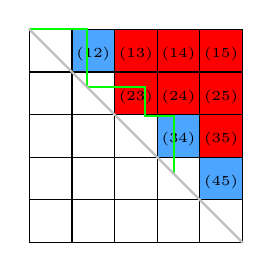
\begin{tikzpicture}[inner sep=0in, outer sep=0in]
                \node (n) {
                \begin{ytableau}
                  \mynone &*(lightblue)\text{\tiny (12)}
                  &*(red)\text{\tiny (13)} &*(red)\text{\tiny (14)}
                  &*(red)
                  \text{\tiny (15)}\\
                  \mynone &\mynone &*(red) \text{\tiny (23)}
                  &*(red)\text{\tiny (24)}
                  &*(red) \text{\tiny (25)}\\
                  \mynone &\mynone &\mynone &*(lightblue) \text{\tiny
                    (34)}
                  &*(red)\text{\tiny (35)} \\
                  \mynone &\mynone &\mynone&\mynone&*(lightblue) \text{\tiny (45)}\\
                  \mynone &\mynone &\mynone&\mynone&\mynone\\
                \end{ytableau}};
              \draw[thick,green] (n.north
              west)--([xshift=2.1em]n.north
              west)--++(0,-2.1em)--++(2.1em,0)--++(0,-1.05em)--++(1.05em,0)--++(0,-2.10em);
              \draw[thick,lightgray] (n.north west)--(n.south east);
              \end{tikzpicture}
              \ \ \
              \scalebox{1.3}{$ 
              \overset{\text{\textcolor{red}{\scriptsize{
                      $\Psi =$ Roots above Dyck
                      path}
                  }
                }}{\text{\textcolor{lightblue}{$\scriptstyle\Delta^+_\ell
                    \setminus \Psi = $ \scriptsize{Non-roots below}}}}
            $}
          \]\pause
          \vspace{-0.1in}
          \begin{block}{Catalan Function~\cite{CH,pany,catalans}}
            For $\Psi$ and $\gamma\in\mathbb Z^\ell$
            $$
            H(\Psi;\gamma)(x) = \prod_{(i,j)\in \textcolor{lightblue}{\Delta^+_\ell
              \setminus \Psi}} (1-R_{ij}) h_\gamma(x)
            $$
          \end{block}\pause
          \begin{itemize}
          \item \(\Psi = \emptyset \implies H(\emptyset;\gamma) =
            s_\gamma\)\pause
          \item \(\Psi =\) all roots \(\implies H(\Psi;\gamma) = h_\gamma\)
          \end{itemize}
        \end{frame}
        \begin{frame}{Catalan functions}
          \begin{block}{\(k\)-Schur root ideal for \(\lambda\)}
            For \(k \in \Z_{\geq 0}\) and \(\lambda = (\lambda_1 \geq
            \ldots \geq \lambda_\ell) \in \Z^\ell\), 
            \begin{align*}
              \Psi = \Delta^k(\lambda)
              & = \{(i,j): j > k-\lambda_i\}\\
              & = \text{root ideal with }k-\lambda_i\text{ \textcolor{lightblue}{non-roots}
                in row }i
            \end{align*}
          \end{block}
          \pause
          \vspace{-0.3in}
          \[
            \Delta^4(3,3,2,2,1,1) = 
\ytableausetup{mathmode, boxsize=.8em,centertableaux}
% ~&*(blue!20)&*(red)&*(red)\\
{\scriptsize
\begin{ytableau}
*(white) 3     &*(lightblue)  &*(red)   &*(red)  &*(red)  &*(red) \\
\mynone & *(white)3 & *(lightblue) & *(red) & *(red)  &*(red)  \\
\mynone &*(white)  & *(white)2 & *(lightblue) & *(lightblue)  &*(red)  \\
\mynone &*(white)  & *(white)  & *(white)2 & *(lightblue) &*(lightblue) \\
\mynone &\mynone  &\mynone  &\mynone  & *(white)1 & *(lightblue) \\
\mynone &\mynone  &\mynone  &\mynone  &*(white)  & *(white) 1
\end{ytableau}
}
\quad
\begin{matrix}
\quad
\\
\quad
\\
\leftarrow \text{row $i$ has $4-\lambda_i$ \textcolor{lightblue}{non-roots}}
\\
\quad
\\
\quad
\end{matrix}
\]
\vspace{-0.2in}
\pause
  \begin{block}{\(k\)-Schur is a Catalan function~\cite{catalans}.}
    For partition \(\lambda\) with \(\lambda_1 \leq k\),
    \[s_\lambda^{(k)} = H(\Delta^k(\lambda);\lambda)\,.\]
  \end{block}
\end{frame}
\begin{frame}{Catalan functions}
  By realizing \(k\)-Schur functions in the framework of Catalan
  functions,~\cite{catalans} proves\pause
  \begin{itemize}
  \item The \(k\)-Schur functions are``shift invariant'', i.e.\ for
    \(\ell = \ell(\lambda)\), \(s_{1^\ell}^\perp
    s_{\lambda+1^\ell}^{(k+1)} = s_\lambda^{(k)}\).\pause
  \item This implies the \(k{+}1\)-Schur expansion of a \(k\)-Schur function has
    positive coefficients. \pause
  \item Also the Schur expansion of a \(k\)-Schur function has positive coefficients.
  \end{itemize}
  \begin{rmk}
   ~\cite{catalans} show results for \(k\)-Schur functions with
   parameter \(t\), but \(t=1\) specialization is necessary for
   Schubert calculus.
  \end{rmk}
\end{frame}
\begin{frame}{Lowering Operators}
  \begin{itemize}
  \item Recall \(K\)-theory/homology of affine Grassmannian
    simultaneously generalizes:
    \begin{itemize}
    \item \(K\)-theory of Grassmannian: \(g_\lambda = \prod_{i < j}
      (1-R_{ij}) k_\lambda\) and \pause
    \item Homology of affine Grassmannian: \(s_\lambda^{(k)} =
      \prod_{(i,j)\in \Delta^+ \setminus \Delta^{k}(\lambda)}
      (1-R_{ij}) h_\lambda\) \pause
    \end{itemize}
  \item Extra ingredient: lowering operators
     \(L_j(h_\lambda) = h_{\lambda-\epsilon_j}\)
            \ytableausetup{boxsize=0.6em}
            \[ L_3\left( \ydiagram{3,1,1}*[*(red)]{0,0,1} \right) =
              \ydiagram{3,1} \ \ L_{1}\left( \ydiagram{3,1,1}*[*(red)]{2+1} \right)
              = \ydiagram{2,1,1}
              \]
  \end{itemize}
\end{frame}
\begin{frame}{Affine \(K\)-Theory Representatives with Raising Operators}
  \begin{definition}
    Let \(\Psi,\lowers \subset \Delta^+_\ell\) be order ideals of
    positive roots and \(\gamma \in \Z^\ell\)\pause, then \[
      K(\Psi;\lowers;\gamma) := \prod_{(i,j) \in \lowers} (1-L_j)
      \prod_{(i,j) \in \Delta^+_\ell \setminus \Psi} (1-R_{ij})
      k_\gamma
    \]
    for \(k_\gamma\) an inhomogeneous analogue of \(h_\gamma\). \pause
  \end{definition}
  \begin{example}
    \(\textcolor{blue}{\text{non-roots of }\Psi\text{ in blue}},
              \text{roots of }\lowers\text{ marked with }\bullet\)
              \begin{columns}
                \begin{column}{0.35\textwidth}
                  \ytableausetup{mathmode,
                    boxsize=1em,centertableaux} \[
                    \begin{ytableau}
                      \mynone &*(lightblue)\text{\tiny (12)}
                      &*(white)
                      &*(white)\bullet &*(white) \bullet \\
                      \mynone &\mynone &*(white) 
                      &*(white) \bullet
                      &*(white) \bullet \\
                      \mynone &\mynone &\mynone &*(lightblue)
                      \text{\tiny (34)}
                      &*(white) \\
                      \mynone &\mynone &\mynone&\mynone&*(lightblue) \text{\tiny (45)}\\
                      \mynone &\mynone &\mynone&\mynone&\mynone\\
                    \end{ytableau}
                  \]
                \end{column}
                \begin{column}{0.65\textwidth}
                  \begin{align*}
                    & K(\Psi;\lowers;54332) \\
                    & = (1-L_{4})^2(1-L_{5})^2
                    \\
                    & \cdot \textcolor{blue}{(1-R_{12})(1-R_{34})(1-R_{45})} k_{54332}
                  \end{align*}
                \end{column}
              \end{columns}
  \end{example}
\end{frame}
% \begin{frame}{Affine \(K\)-Theory Representatives with Raising
%     Operators}
%   \begin{definition}
%     The \emph{\(k\)-Schur root ideal}, \(\Delta^{(k)}(\lambda)\) is the
%     unique root ideal with \(\lambda_i + \#\)non-roots in row \(i =
%     k\).
%   \end{definition}
%   \begin{example}
%   \(k=4, \lambda = 332111\)
%               \[
%               \Delta^{(4)}(332111) = 
%               {\footnotesize
%                 \begin{ytableau}
%                   *(white) 3     &*(lightblue)  &*(red)   &*(red)  &*(red)  &*(red) \\
%                   \mynone & *(white)3 & *(lightblue) & *(red) & *(red)  &*(red)  \\
%                   \mynone & \mynone  & *(white)2 & *(lightblue) & *(lightblue)  &*(red)  \\
%                   \mynone & \mynone  & \mynone  & *(white)1 & *(lightblue) &*(lightblue) \\
%                   \mynone &\mynone  &\mynone  &\mynone  & *(white)1 & *(lightblue) \\
%                   \mynone &\mynone  &\mynone  &\mynone  & \mynone  & *(white) 1
%                 \end{ytableau}
%               }
%               \leftarrow\,\text{\small{4 - 2 non-roots}}
%               \quad
%             \]
%             \end{example}
% \end{frame}
\begin{frame}{Affine \(K\)-Theory Representatives with Raising Operators}
  \begin{block}{Answer (Blasiak-Morse-S., 2020)}
    \pause For \(K\)-homology of affine Grassmannian, \(f_\lambda = g_\lambda^{(k)} :=
    K(\Delta^{(k)}(\lambda); \Delta^{(k+1)}(\lambda);\lambda)\) since
    this family has the correct structure constants. 
  \end{block}
  \pause
  \begin{example}
\(              g_{332111}^{(4)} = \){\footnotesize
                \begin{ytableau}
                  *(white) 3     &*(lightblue)  &*(white)   &*(white) \bullet  &*(white) \bullet  &*(white) \bullet \\
                  \mynone & *(white)3 & *(lightblue) & *(white) & *(white) \bullet  &*(white) \bullet  \\
                  \mynone &\mynone  & *(white)2 & *(lightblue) & *(lightblue)  &*(white)  \\
                  \mynone &\mynone  & \mynone  & *(white)1 & *(lightblue) &*(lightblue) \\
                  \mynone &\mynone  &\mynone  &\mynone  & *(white)1 & *(lightblue) \\
                  \mynone &\mynone  &\mynone  &\mynone  &\mynone & *(white) 1
                \end{ytableau}
              }
\(\textcolor{blue}{\Delta^+ \setminus \Psi = \Delta^+_6 \setminus \Delta^{(4)}(332111)},
\lowers = \Delta^{(5)}(332111)\)
\end{example}
\end{frame}
\begin{frame}{Property and Further Work}
  \begin{theorem}[Blasiak-Morse-S., 2020]
     \pause The \(g_\lambda^{(k)}\) are ``shift
        invariant'', i.e.\ for \(\ell = \ell(\lambda)\)
      \[
        G_{1^\ell}^\perp g_{\lambda+1^\ell}^{(k+1)} = g_\lambda^{(k)}
      \]
  \end{theorem}\pause
  \begin{theorem}[Blasiak-Morse-S., 2020]
    The \(g_\lambda^{(k)}\) ``branching coefficients'' are alternating
    by degree, i.e.\ the \(b_{\lambda \mu}^{(k)}\) in \[
      g_\lambda^{(k)} = \sum_\mu b_{\lambda\mu}^{(k)} g_\mu^{(k+1)}
    \]
    satisfy \((-1)^{|\lambda|-|\mu|} b_{\lambda\mu}^{(k)} \in \Z_{\geq
    0}\). 
  \end{theorem}
  \end{frame}
\begin{frame}{Future Directions}
    For \(G_\lambda^{(k)}\) an affine Grothendieck polynomial (dual to \(g_\lambda^{(k)}\)),\pause
    \begin{enumerate}
    \item Combinatorially describe dual ``Pieri rule'': \(G_{1^r}^\perp g_\lambda^{(k)} = \sum_\mu
      ?? g_\mu^{(k)} \iff G_{1^r} G_\mu^{(k)} = \sum_\lambda ?? G_\lambda^{(k)}\),  \(1 \leq r \leq k\).\pause
    \item Combinatorially describe branching coefficients: \(g_\lambda^{(k)} =
      \sum_\mu ?? g_\mu^{(k+1)}\).\pause
    \item Combinatorially describe \(g_\lambda^{(k)} = \sum_\mu ??
      s_\mu^{(k)}\).%\pause
    % \item Prove the image of \(\G_w^Q\) under \(K\)-theoretic Peterson isomorphism
    %   for all \(w \in S_{k+1}\).
    \end{enumerate}
\end{frame}
\begin{frame}{References}
  Thank you!
  \begin{bibdiv}
  \begin{biblist}
    \bib{catalans}{article}{
      author={Blasiak, Jonah}
      author={Morse, Jennifer}
      author={Pun, Anna}
      author={Summers, Daniel}
      title={Catalan Functions and \(k\)-Schur Positivity}
      year={2019}
      journal={Journal of the AMS}
    }
    \bib{CH}{thesis}{
      author={Chen, Li-Chung}
      title={Skew-linked partitions and a representation theoretic
        model for \(k\)-Schur functions}
      type={Ph.D. thesis}
      year={2010}
      ios={U.C. Berkeley}
    }
    \bib{lss}{article}{
      author={Lam, Thomas}
      author={Schilling, Anne}
      author={Shimozono, Mark}
      title={K-theory Schubert calculus of the affine
        Grassmannian}
      year={2010}
      journal={Compositio Math.}
      volume={146}
      pages={811--852}
    }
    \bib{morse}{article}{
      author={Morse, Jennifer}
      title={Combinatorics of the K-theory of affine
        Grassmannians}
      year={2011}
      journal={Advances in Mathematics}
    }
    \bib{pany}{article}{
      author={Panyushev, Dmitri I.}
      title={Generalised Kostka-Foulkes polynomials and cohomology of
        line bundles on homogeneous vector bundles}
      journal={Selecta Math. (N.S.)}
      volume={16}
      year={2010}
      number={2}
      pages={315--342}
    }
  \end{biblist}
  \end{bibdiv}
\end{frame}
\end{document}
%%% Local Variables:
%%% mode: latex
%%% TeX-master: t
%%% End:
